\documentclass{article}

\usepackage[left=2.5cm, right=2.5cm, top=2.5cm, bottom=2.5cm]{geometry}
\usepackage{graphicx}
\usepackage{physics}
\usepackage{algpseudocode}
\usepackage{subcaption}


\title{Exercise 1, TFY4235 Computational physics}
\author{Martin K. Johnsrud}
\vspace{-8ex}
\date{}

\begin{document}
    \maketitle
    \section*{Introduction}
        The goal of this exercise is to simulate particles as flat, hard disks in a square, 2D container. This is done with a event-driven simulation, as described in the exercise~\cite{exercise}. This is implemented in Python, using the built-in library heapq. The simulation is used to first tested with scenarios we know the outcome of, then used to demonstrate the Maxwell-Boltzmann distribution and to investigate the effect of a large, heavy disk hitting a large number of small, inert particles.
    
    \section*{Implementation}
        The main engine of the code is the function \verb|run_loop()| in \verb|utillities.py|. It follows the algorithm, as laid out in~\cite{exercise}, using the objects:
        \begin{itemize}
            \item \verb|particles|, a numpy array with the position and velocity of all the particles.
            \item \verb|t|, a list where \verb|t[i]| is the time of collision number \verb|i|.
            \item \verb|collisions|, a priority queue containing a list for each collision. The list has the time of the collision, the index of the particle(s) involved, and the type of collision it is. The list is sorted by the time of the collision.
            \item \verb|last_collided|, a list of when each particle was involved in a collision.
        \end{itemize}
        The function takes the parameters for the simulation, \verb|(N, T, radii, masses, xi)|, which is resp. the number of particles, number of time steps to be executed, a list with the radii of the particles, a list of the masses, and the restitution coefficient $\xi$. It also takes a function \verb|init|, which is used to set the initial distribution of particles. 
        
        When the particles are initiated, a while loop executes the algorithm as described in \cite{exercise}. The next collision is found by the \verb|heappop| method of \verb| collisions|. The list \verb|last_collided| is used to check if the next collision is valid. The function \verb|exectue_collision| translates the particles forward in time, finds the new velocities for the particles involved in the collision, as shown in ~\cite{exercise}, before finally finding the new collisions, given the updatet positions and velocities. The \verb|run_loop| function can be given the argument \verb|TC=True|. Then, it runs a TC-model, as described in ~\cite{TC}. If the function is passed the argument \verb|condition=func|, it will check the function \verb|func| at regular intervals. This makes it possible to exit the loop early. It is used to run the simulation until $10\%$ of the energy is remaining, as described later in the report.

        \verb|profile.ipynb| shows the profiling of \verb|run_loop|, and the subroutines that takes the most time. This shows that it is the loop that pushes the next collisions to the priority queue that is the bottle neck. A large (HOW LARGE?) speedup was found by rewriting the function that finds the collisions. The notebook \verb|profile_old.ipynb| shows the time used by the old version. The old version of the functions took the index \verb|i| of the particle in question, then found if and when it was to collide with all other collisions, and returned this time as a list. The new version utilizes the fact that everything is contained in numpy-arrays. It does the same operations as the old function, only on arrays instead of single elements. This is done by using masks. An array of booleans can serve as indecies, so \verb|lst[np.arange(N) != i]| gives an array with all the elements of \verb|lst[i]|. The profiling show that while most of the time went to the calculation of the next collision, it now goes to pushing to the \verb|collisions|-heap.

    \section*{Tests}
        Several functions were developed to test the accuracy of the simulation. First, one particle, starting at in the middle of the box, all the way to the left, and with a velocity with at $45^\circ$ to the $x$-axis should move in a titled rectangle. With $\xi=1$ it should also conserve energy. Figure \ref{single particle} shows that this is still the case after $10,000$ events.

        \begin{figure}
            \begin{subfigure}{.35\textwidth}
                \includegraphics[width=0.49\textwidth]{../plots/test_case_one_particle/particle-4.pdf}
                \includegraphics[width=0.49\textwidth]{../plots/test_case_one_particle/particle-3.pdf}
                \includegraphics[width=0.49\textwidth]{../plots/test_case_one_particle/particle-2.pdf}
                \includegraphics[width=0.49\textwidth]{../plots/test_case_one_particle/particle-1.pdf}
                \caption{One ball being simulated. after $10 000$ steps, it still follows a regular pattern.}
                \label{single particle}
            \end{subfigure}
            \begin{subfigure}{.65\textwidth}
                \includegraphics[width=.8\textwidth]{../plots/test_case_one_particle/energy.pdf}
                \caption{cap2}
                \label{lab2}
            \end{subfigure}
        \end{figure}
        
        To test the validity of the particle collision, one small, light particle is sent towards a single, large and heavy particle, with varying impact parameters. The relationship between the impact parameter is is (ref til goldstein, begunn hvorfor det blir cos) $\dv{s}{\theta} = a / 2 \sin(\theta / 2)$. The result is shown i Figure \ref{scattering}, and is in good agreement with the theory. Lastly, the energy from a simulation of $N$ particles over $T$ events is shown in


        \begin{figure}
            \centering
            \includegraphics[width=0.8\textwidth]{../plots/test_case_collision_angle/collision_angle.pdf}
            \caption{The }
            \label{scattering}
        \end{figure}

        \begin{figure}
            \centering
            \includegraphics[width=0.35\textwidth]{../plots/test_case_many_particles/test_case_many_particles.pdf}
            \includegraphics[width=0.54\textwidth]{../plots/test_case_many_particles/energy.pdf}
            \caption{On the left is a snapshot of the particles. The arrows represent the velocities. On the right, the energy is plotted as a function of events. The energy loss can be seen to be negligible.}
        \end{figure}

        \section*{Results}
            As the system equilibrates, it should reach the Maxwell-Boltzmann distribution, which in 2D is
            \begin{equation*}
                f(v) = \frac{m v}{T} \exp \left(-\frac{m v^2}{2 T}\right),
            \end{equation*}
            when using units in which $k_b = 1$. The equipartition theorem gives the temperature $T = E$ in 2D. Figure \ref{problem1 av vel} was used to find a good starting point for when the simulation has reach equilibrium. After that, the simulation is sampled every $N$ event, where $N$ is the number of particles. This ensures somewhat independent samples. Figure \ref{problem1 dist} shows the velocity distribution, compared to the Maxwell Boltzmann distribution. 
            \begin{figure}
                \centering
                \includegraphics[width=0.8\textwidth]{../plots/problem1/vel_dist.pdf}
                \caption{The velocity distribution is a good fit with the Maxwell-Boltzmann distribution, shown as a blue line.}
                \label{problem1 dist}
            \end{figure}
            \begin{figure}
                \centering
                \includegraphics[width=0.8\textwidth]{../plots/problem1/v_av.pdf}
                \caption{Average velocity, as a function of collisions. The distribution reaches equilibrium around $6000$ collisions, or $3N$}
                \label{problem1 av vel}
            \end{figure}

            Next, two different types of particles are simulated, one with a mass of $1$, the other with a mass of $4$. test

            \begin{figure}
                \centering
                \includegraphics[width=0.95\textwidth]{../plots/problem2/vel_dist.pdf}
                \caption{The velocity distribution of the particles with $m=1$ and $m=4$ is show left and right, resp. and compared to the Maxwell-Boltzmann distribution.}
                \label{problem2 dist}
            \end{figure}

            By setting the elasticity parameter (?) $\xi$ to different values, the way the system approaches equilibrates changes.

            \begin{figure}
                \centering
                \hspace{-5mm}
                \includegraphics[width=0.35\textwidth]{../plots/problem3/xi_0/energy_ex3.pdf}
                \hspace{-4mm}
                \includegraphics[width=0.35\textwidth]{../plots/problem3/xi_1/energy_ex3.pdf}
                \hspace{-4mm}
                \includegraphics[width=0.35\textwidth]{../plots/problem3/xi_2/energy_ex3.pdf}
                \hspace{-5mm}
                \caption{The average energy, as a function of time, of resp. $\xi=1$, $\xi=0.9$ and $\xi=0.8$.}
                \label{problem2 dist}
            \end{figure}

            To simulate the impact of a projectile, one disk is placed at $\vec x = (0.5, 0.75)$, and given a velocity of $v = (0, -20)$. The lower half of the square box is filled with small, light particles. The impact from the large disk into the densely packed disks will create a crater. To investigate the effect of the mass and radius on the size of the crater, the size of the crater must be measured. This is done by laying a grid with with a spacing $\Delta x$, and searching through each cell if there is a disk inside it. The process for checking if a disk is inside each square cell is illustrated in figure \ref{cheack if disk is inside}. Then, the size of the crater is given by $s = m \Delta x^2$, where $m$ is the number of unoccupied cells. This method relies on choosing a cell size $\Delta x$ large enough so that only cells within the crater are empty. This is done by inspecting the result, and comparing it to a plot of the crater.

            \begin{figure}[ht]
                \centering
                \includegraphics[width=0.8\textwidth]{figure.pdf}
                \caption{Checking if a disk of radius $R$ is inside of a square of side length $\Delta x$, is equivalent to checking if the center of the disk is inside the shape on the left side. Thus, the task is reduced to checking if the center is inside the larger square of side lengths $R + 2 \Delta x$, but not at the corners, or inside one of the circles of radius $R$ centered at the corners of the square.}
                \label{cheack if disk is inside}
            \end{figure}

            To avoid inelastic, which was first observed when the projectile was approa ching the bottom of the box, the simulation was implemented as at TC-model as described in~\cite{TC}. Good results, without inelastic collapse, were found with $t_c = 10^{-8}$.

            \begin{figure}
                \centering
                \includegraphics[width=0.40\textwidth]{../plots/problem4/crater8.pdf}
                \includegraphics[width=0.30\textwidth]{../plots/problem4/particles8.pdf}
            \end{figure}

            To investigate the effect of the size of projectile on the crater, the simulation is run 10 times, using projectiles with different radius. The mass of the projectile is proportional to $R^2$, so that the density is constant. Figure \ref{crater size} shows the size of the crater, 

            \begin{figure}
                \centering
                \includegraphics[width=0.8\textwidth]{../plots/problem4/crater_size.pdf}
                \caption{The size of the crater, as a function of the radius of the incoming projectile.}
                \label{crater size}
            \end{figure}

    \bibliography{report}
    \bibliographystyle{plain}   
\end{document}